\documentclass[tikz,border=4pt]{standalone}
\usepackage{ctex}
\usepackage{amsmath}
\usetikzlibrary{arrows.meta}

% p8-01: 函数三种表示法示意图（图象法——y=2x 的图象）
\begin{document}
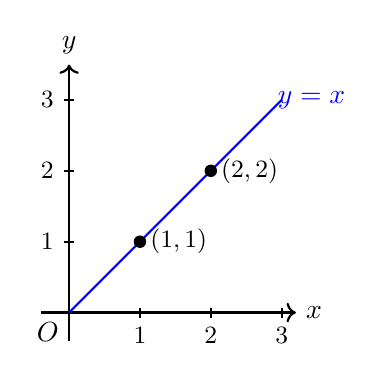
\begin{tikzpicture}[scale=0.9, thick]
  % 坐标轴
  \draw[->] (-0.4,0) -- (3.2,0) node[right] {$x$};
  \draw[->] (0,-0.4) -- (0,3.5) node[above] {$y$};
  \node[below left] at (0,0) {$O$};

  % 刻度
  \foreach \x in {1,2,3} {
    \draw (\x, 2pt) -- (\x, -2pt) node[below] {\small$\x$};
  }
  \foreach \y in {1,2,3} {
    \draw (2pt,\y) -- (-2pt,\y) node[left] {\small$\y$};
  }

  % 函数 y=x 的图象（简单正比例函数示例）
  \draw[blue, thick] (0,0) -- (3,3);

  % 标记几个点
  \fill (1,1) circle (2.5pt);
  \node[right] at (1,1) {\small$(1,1)$};
  \fill (2,2) circle (2.5pt);
  \node[right] at (2,2) {\small$(2,2)$};

  % 函数标签
  \node[right, blue] at (2.8, 3) {$y=x$};
\end{tikzpicture}
\end{document}
